{
\renewcommand{\thechapter}{\arabic{chapter}N}
\setcounter{chapter}{15}
\chapter{Exame normal 2015/16}
\section{Pergunta 1}
Uma associação reflexiva representa:
\begin{enumerate}[label=\alph*.]\itemsep0em
    \item uma associação que representa uma relação ``é um''/``é uma''
    \item uma associação envolvendo outra associação
    \item Não quero responder
    \item \textbf{uma associação envolvendo a mesma classe mais do que uma vez \greencheckmark}
    \item uma associação entre uma classe e a sua super-classe
\end{enumerate}

\section{Pergunta 2}
Se a 3ª Forma Normal pode ser descrita como ``cada atributo depende da chave, de toda a chave e de nada além da chave'', a 1FN seria descrita como:
\begin{enumerate}[label=\alph*.]\itemsep0em
    \item cada atributo depende da chave e de nada para além da chave
    \item \textbf{cada atributo depende da chave \greencheckmark}
    \item Não quero responder
    \item cada atributo depende da chave, de toda a chave
    \item cada atributo dependen de nada para além da chave
\end{enumerate}

\section{Pergunta 3}
Qual a expressão em álgebra relacional equivalente à seguinte consulta SQL:
\begin{lstlisting}[language=SQL]
SELECT c1, MAX(c2) FROM T1 NATURAL JOIN T2 WHERE c3=5 GROUP BY c1;
\end{lstlisting}
\begin{enumerate}[label=\alph*.]\itemsep0em
    \item $\pi_{c1, \text{MAX}(c2)}(\sigma_{c3=5}(T1 \naturaljoin T2))$ \greencheckmark
    \item Não quero responder
    \item $\pi_{c1,\text{MAX}(c2)}(\sigma_{c3=5}(T1) \naturaljoin T2)$
    \item $\sigma_{c3=5}(\pi_{c1,\text{MAX}(c2)}(T1 \naturaljoin T2))$
    \item $\text{MAX}_{c2}(\pi_{c1}(\sigma_{c3=5}(T1) \naturaljoin T2))$
\end{enumerate}

\section{Pergunta 4}
Tendo a chave primária já definida, como se define uma segunda chave candidata em LDD-SQL?
\begin{enumerate}[label=\alph*.]\itemsep0em
    \item Não quero responder
    \item Com a cláusula \texttt{PRIMARY KEY}
    \item Com a cláusula \texttt{FOREIGN KEY}
    \item \textbf{Com a cláusula \texttt{UNIQUE} \greencheckmark}
    \item Com uma das cláusulas \texttt{PRIMARY KEY} ou \texttt{UNIQUE}
\end{enumerate}

\section{Pergunta 5}
Uma vista
\begin{enumerate}[label=\alph*.]\itemsep0em
    \item pode ser usada como qualquer tabela
    \item Não quero responder
    \item \textbf{pode ser usada como qualquer tabela, exceto se só permitir inserção de registos se não juntar várias tabelas \greencheckmark}
    \item pode ser usada como qualquer tabela, exceto para operações de \texttt{DELETE}
    \item só pode ser usada como tabela de for materializada
\end{enumerate}

\section{Pergunta 6}
As linguagens PSM:
\begin{enumerate}[label=\alph*.]\itemsep0em
    \item permitem que o sistema de gestão de bases de dados execute código escrito em linguagens de programação (ex. C, Java)
    \item Não quero responder
    \item \textbf{permitem a implementação em bases de dados relacionais de operações de natureza não declarativa (isto é, dificilmente implementáveis em SQL) \greencheckmark}
    \item facilitam a utilização em linguagens de programação de persistent stored modules escritos em SQL
    \item permitem usar instruções de linguagens de programação (ex. C, Java) em \texttt{SELECT}s
\end{enumerate}

\section{Pergunta 7}
Um ponto de verificação (checkpoint) serve para:
\begin{enumerate}[label=\alph*.]\itemsep0em
    \item Não quero responder
    \item \textbf{definir um momento em que a base de dados está consistente \greencheckmark}
    \item criar uma cópia de segurança
    \item registar um commit
    \item determinar quais as transações ainda incompletas
\end{enumerate}

\section{Problema 8}
A forma tradicional de implementar escalabilidade dos servidores de base de dados:
\begin{enumerate}[label=\alph*.]\itemsep0em
    \item é a vertical, que consiste implementação de vários níveis de servidores para armazenar todos os dados
    \item é a horizontal, que consiste na partição dos dados, o que implica a compra de hardware mais poderoso
    \item é a horizontal, que consiste na partição dos dados, o que permite suportar a base de dados em hardware menos poderoso
    \item Não quero responder
    \item \textbf{é a vertical, que consiste na compra de hardware mais poderoso para armazenar todos os dados \greencheckmark}
\end{enumerate}

\section{Problema 9}
Uma diferença essencial entre uma base de dados e um armazém de dados é que
\begin{enumerate}[label=\alph*.]\itemsep0em
    \item ambos optimizam a velocidade de acesso de formas diferentes: a primeira minimiza a redundância enquanto o segundo a maximiza
    \item ambos otimizam a velocidade de acesso de formas diferentes: a primeira maximiza a redundância enquanto o segundo a minimiza
    \item \textbf{a primeira minimiza a redundância enquanto que o segundo utiliza a redundância para otimizar a velocidade de consulta \greencheckmark}
    \item Não quero responder
    \item a primeira maximiza a redundância enquanto que o segundo a minimiza para otimizar a velocidade de consulta
\end{enumerate}

\section{Pergunta 10}
A avaliação do desempenho de um algoritmo num problema de previsão, costuma envolver a divisão dos dados em
\begin{enumerate}[label=\alph*.]\itemsep0em
    \item 10 sub-conjuntos, 5 para obter o modelo e os restantes para medir o seu desempenho preditivo
    \item 2 subconjuntos, em que o primeiro é usado para induzir o modelo, sendo o seu desempenho medido no conjunto completo
    \item 5 sub-conjuntos, usando o primeiro para obter o modelo, e avaliando-o no segundo; depois induzir outro modelo no segundo, e avaliando-o no terceiro; e assim sucessivamente
    \item \textbf{2 sub-conjuntos, em que um serve para obter o modelo e outro para medir o seu desempenho preditivo \greencheckmark}
    \item Não quero responder
\end{enumerate}

\section*{Informação}
Considere o esquema relacional $R(A,B,C,D,E,F,G,H)$ e as seguintes dependências funcionais:
\begin{alignat*}{2}
    & A,B,C && \rightarrow D,G,H\\
    & F     && \rightarrow B\\
    & B     && \rightarrow E\\
    & G     && \rightarrow H    
\end{alignat*}

\section{Pergunta 11}
Qual das seguintes dependências funcionais não pode ser obtida?
\begin{enumerate}[label=\alph*.]\itemsep0em
    \item \label{itm:2016N-11-a} $A,F,C \rightarrow D$
    \item \label{itm:2016N-11-b} $A,F \rightarrow E$
    \item \label{itm:2016N-11-c} Não quero responder
    \item \label{itm:2016N-11-d} \textbf{$A,F \rightarrow D$ \greencheckmark}
    \item \label{itm:2016N-11-e} $A,C,D \rightarrow D$
\end{enumerate}
O item \ref{itm:2016N-11-a} é possível se considerarmos $\{A,F,C\}^+=\{A,B,C,F\}^+=\{A,B,C,D,F,G,H\}^+$.\\
O item \ref{itm:2016N-11-b} é possível se considerarmos $\{A,F\}^+=\{A,B,F\}^+=\{A,B,E,F\}^+$.\\
O item \ref{itm:2016N-11-d} não é possível dado que $\{A,F\}^+=\{A,B,F\}^+=\{A,B,E,F\}^+=\{A,B,E,F\}$.\\
O item \ref{itm:2016N-11-e} é possível dado que é trivial.

\section{Pergunta 12}
\textbf{Verifique se relação $R$ se encontra na forma normal de Boyce-Codd. Justifique.}

\ansseparator

Uma relação está na forma normal de Boyce-Codd (BCNF) sse, para toda a dependência funcional não-trivial $\overline{A} \rightarrow \overline{B}$, $\overline{A}$ é uma superchave.

Dado que $\{G\}^+=\{G,H\}^+=\{G,H\}$, pode-se verificar que $\{G\}$ não é uma superchave, dado que o seu fecho $\{G\}^+=\{G,H\}$ não inclui todos os atributos. Assim, $R$ não está na BCNF.

\section{Pergunta 13}
Construa um modelo concetual de dados em UML para armazenar a informação associada a uma rede de lojas comerciais. Indique todas as restrições que possam ser úteis para a construção da base de dados.

Os responsáveis por uma rede de lojas comerciais pretendem construir um sistema informático para gerir toda a informação associada às lojas, aos produtos, aos fornecedores e aos clientes. O sistema deve permitir registar informação sobre os produtos, nomeadamente o nome, uma descrição, o preço de venda atual (que é o mesmo em todas as lojas), e a categoria do produto (p.e. alimentação, limpeza, congelados, etc). Importa também permitir o registo dos diversos fornecedores que disponibilizam cada um dos produtos, bem como o preço praticado por cada um. Cada produto pode ser disponibilizado por mais do que um fornecedor.

O sistema deve manter informação detalhada sobre os fornecedores. As encomendas de produtos aos fornecedores são geridas centralmente e é necessário registar, para cada encomenda, qual o fornecedor, quais os produtos encomendados, e qual a quantidade e preço de cada um.

Sobre cada loja, deve ser possível registar, para além dos contactos e localização física da loja, os produtos e respetiva quantidade existente em armazém. Importa também registar as compras realizadas na loja por cada cliente. O sistema deve permitir manter um registo global de todos os clientes e sobre cada compra é necessário registar a loja onde se realizou e qual o produto (e preço) do produto comprado.

\ansseparator

\begin{center}
    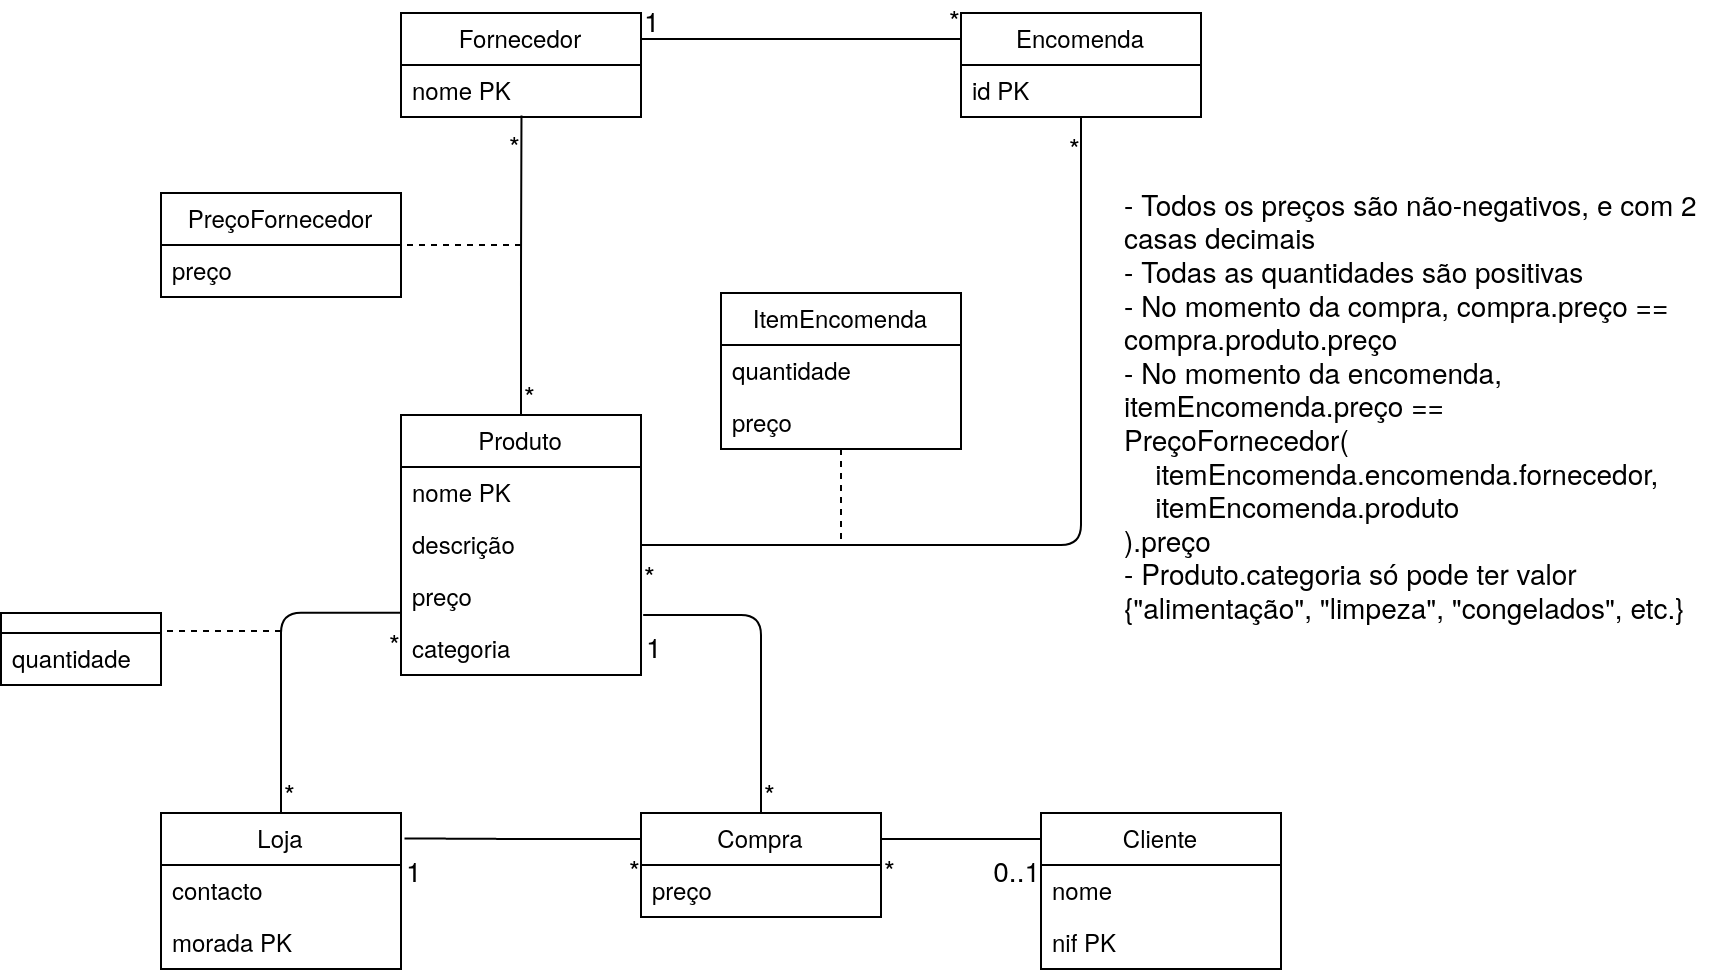
\includegraphics[scale=0.263]{2016N_13.png}
\end{center}

\newpage
\section*{Informação}

Os estudantes da FEUP decidiram organizar a sua rede social usando uma base de dados com o seguinte modelo relacional:

\begin{lstlisting}[numbers=none]
Curso (ID, nome)
Estudante (ID, nome, curso->Curso, anoCurricular)
Amizade (ID1->Estudante. ID2->Estudante)
\end{lstlisting}

O estudante com ID1 é amigo do estudante com ID2. Como as amizades são mútuas, se (176, 9) está na tabela \texttt{Amizade}, (9,176) também está.

A execução das interrogações deve ser feita numa base de dados SQLite criada com as instruções SQL existentes no ficheiro \texttt{redesocial.sql}.

Deve escrever a interrogação usando SQL. Como as interrogações serão executadas usando SQLite, devem ser compatíveis com a sintaxe SQL suportada pelo SQLite.

Para cada interrogação é apresentada a resposta esperada para a base de dados associada ao ficheiro \texttt{redesocial.sql}. Esta informação deve ser utilizada para validar a resposta antes de a submeter. Por omissão, a saída do SQLite só apresenta colunas com 10 caracteres. O número de caracteres de cada coluna pode ser ajustado utilizando o comando:

\begin{lstlisting}[language=SQL,numbers=none]
.width <num caracteres coluna 1> < num caracteres coluna 2>...
\end{lstlisting}

\section{Pergunta 14}
Liste o nome de cada estudante inscrito no 3º ano curricular, seguido do nome do curso em que está inscrito.
\begin{center} \begin{tabular}{l | l}
    \textbf{Estudante} & \textbf{Curso} \\ \hline
    Carla Silva        & MIEIC          \\
    Joana Teixeira     & MIEEC          \\
    Carlos Rodrigues   & MIEIC          \\
    Sergio Carvalho    & MIEEC
\end{tabular} \end{center}
\ansseparator
\lstinputlisting[language=SQL]{2016N_14.sql}

\section{Pergunta 15}
Liste o nome dos estudantes com mais de 3 amigos.
\begin{center} \begin{tabular}{l}
    \textbf{nome}    \\ \hline
    Carla Silva      \\
    Mafalda Pimentel \\
    Gabriel Maria
\end{tabular} \end{center}
\lstinputlisting[language=SQL]{2016N_15.sql}

\section{Pergunta 16}
Liste o nome e ano curricular dos estudantes que só têm amigos do mesmo ano curricular. Devolva os resultados ordernados por ano curricular e depois por nome dentro de cada ano curricular. Não devem ser devolvidos os estudantes que não têm amigos.
\begin{center} \begin{tabular}{l | l}
    \textbf{Nome}    & \textbf{Ano Curricular} \\ \hline
    Ana Lopes        & 1                       \\
    Diogo Teixeira   & 2                       \\
    Maria Felisberta & 2                       \\
    Carlos Rodrigues & 3
\end{tabular} \end{center}
\lstinputlisting[language=SQL]{2016N_16.sql}

\section{Pergunta 17}
Liste os identificadores dos amigos em 3º grau do Miguel Sampaio. Um amigo em 3º grau é um amigo de um amigo de um amigo. A listagem não deve ter tuplos repetidos.
\begin{center} \begin{tabular}{l}
    \textbf{ID} \\ \hline
    201101661   \\
    201101689   \\
    201101782   \\
    201101934 
\end{tabular} \end{center}
\lstinputlisting[language=SQL]{2016N_17.sql}

\section{Pergunta 18}
Indique o nome e ano curricular do(s) estudante(s) que tem o maior número de amigos.
\begin{center} \begin{tabular}{l | l}
    \textbf{nome} & \textbf{anoCurricular} \\ \hline
    Gabriel Maria & 1
\end{tabular} \end{center}
\lstinputlisting[language=SQL]{2016N_18.sql}

\section{Pergunta 19}
Crie um gatilho que, na inserção de um estudante, o torne amigo de todos os outros estudantes do mesmo curso. Não se esqueça que as amizades são mútuas. As amizades inseridas devem ser apenas entre pessoas distintas, ou seja, um estudante não pode ser considerado amigo de si próprio.
\lstinputlisting[language=SQL]{2016N_19.sql}

}
